\subsubsection{Logic contracts}
In this section we show how the logic contracts of \textit{Soldino} work. These contracts implement a major part of the business logic, defining:
\begin{itemize}
	\item inputs validation mechanics;
	\item events to be emitted on the blockchain when a state change is made;
	\item communication with each other.
\end{itemize}
Since logic contracts are upgradeable, every logic contract has a \texttt{ContractManager} state variable, used to get the latest address of another contract. In this way the coupling between logic contract is minimum and there's no need to maintain correct references in each logic contract.\\
However each \texttt{xLogic} contract has a direct reference to its \texttt{xStorage} contract because the latter is immutable.
\pagebreak
\paragraph{UserLogic}\mbox{}\\

\noindent This contract provides an interface to comunicate with the \texttt{UserStorage} contract. \texttt{addCitizen} and \texttt{addBusiness} functions add a new user and set its type depending on which function is called.
\begin{figure}[H]
	\centering
	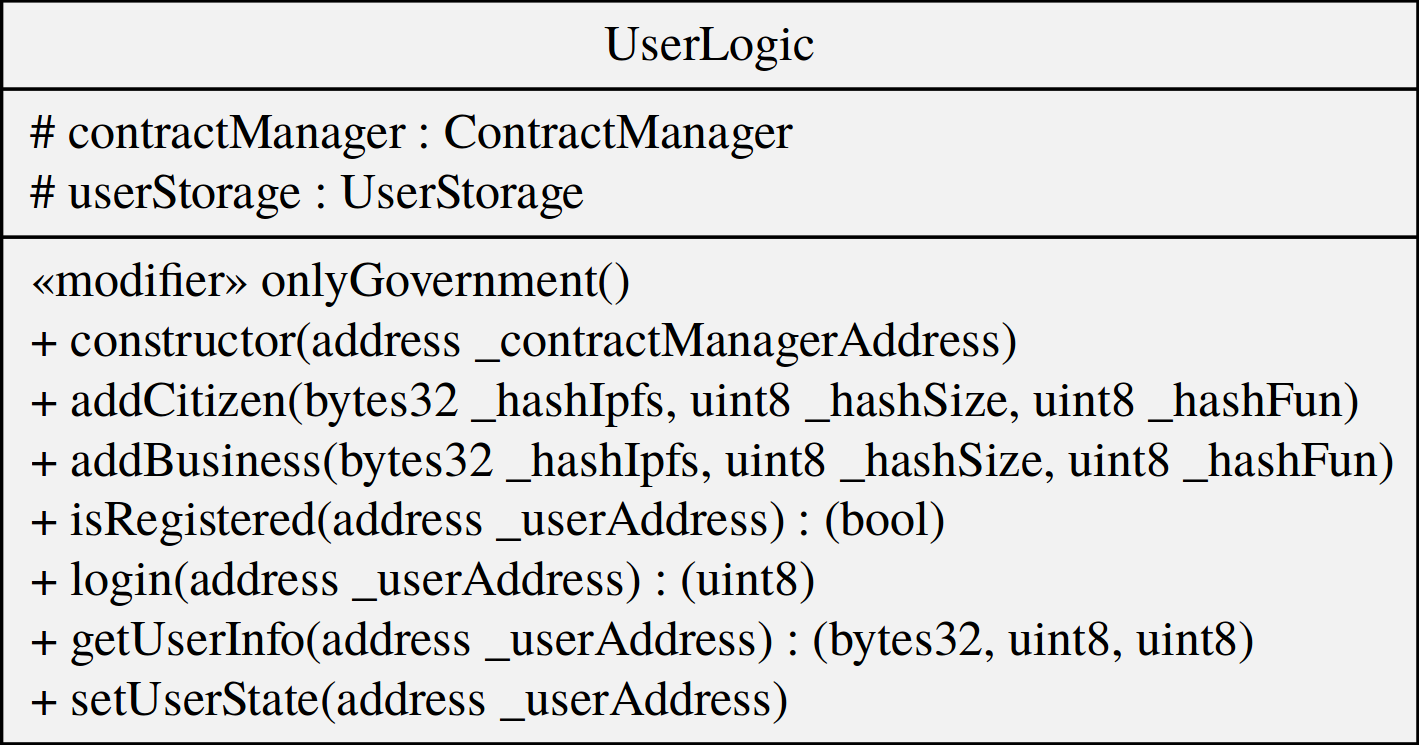
\includegraphics[scale=0.20]{res/images/solidity/userlogic.png}
	\caption{class diagram of the UserLogic contract}
\end{figure}

\paragraph{ProductLogic}\mbox{}\\

\noindent This contract allows business to insert new products, modify or delete exiting ones. Obviously, only businesses can insert products in \textit{Soldino}: to comply this requirement \texttt{ProductLogic} defines the modifier \texttt{onlyBusiness} which checks if the address of the contract that is trying to insert a product is a business. Furthermore, products can be modified and deleted only by their sellers and the modifier \texttt{onlyProductOwner} is responsible for that.
\begin{figure}[H]
	\centering
	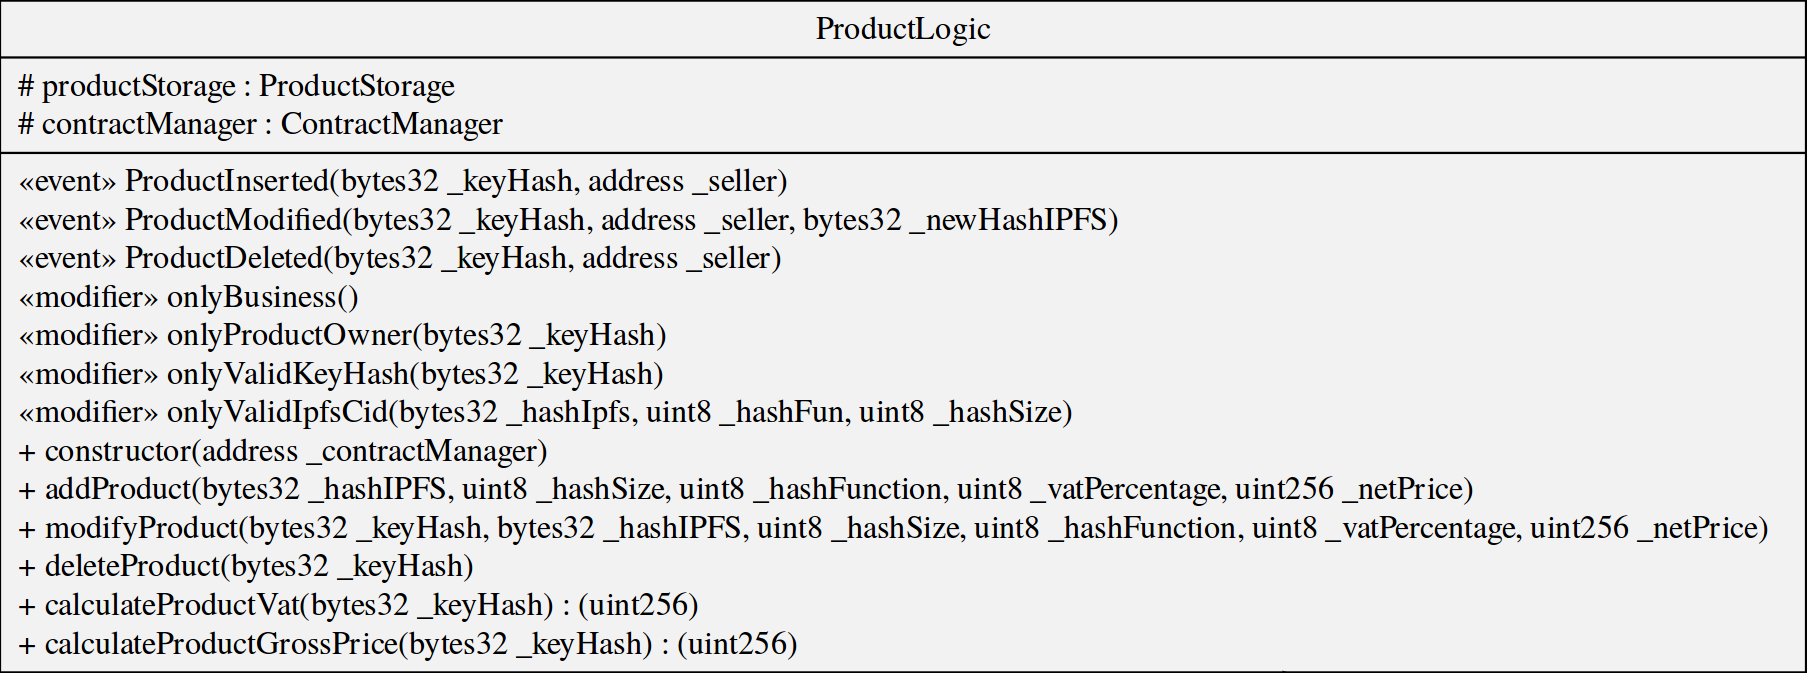
\includegraphics[scale=0.25]{res/images/solidity/productlogic.png}
	\caption{class diagram of the ProductLogic contract}
\end{figure}
\pagebreak
\paragraph{VatLogic}\mbox{}\\

\noindent This contract defines the logic to interact with the \texttt{VatStorage} contract. 
Its function \texttt{refundVat} makes sure that only the government can refund the VAT to a business, thanks to the attached modifier \texttt{onlyGovernment}.\\
In order to store VAT movements broken down by business and quarter, the function \texttt{createVatKey} computes a valid key for the map stored in \texttt{VatStorage} using the address of the business and the string representing the quarter in format \texttt{"year-quarterNumber"}. 
\begin{figure}[H]
	\centering
	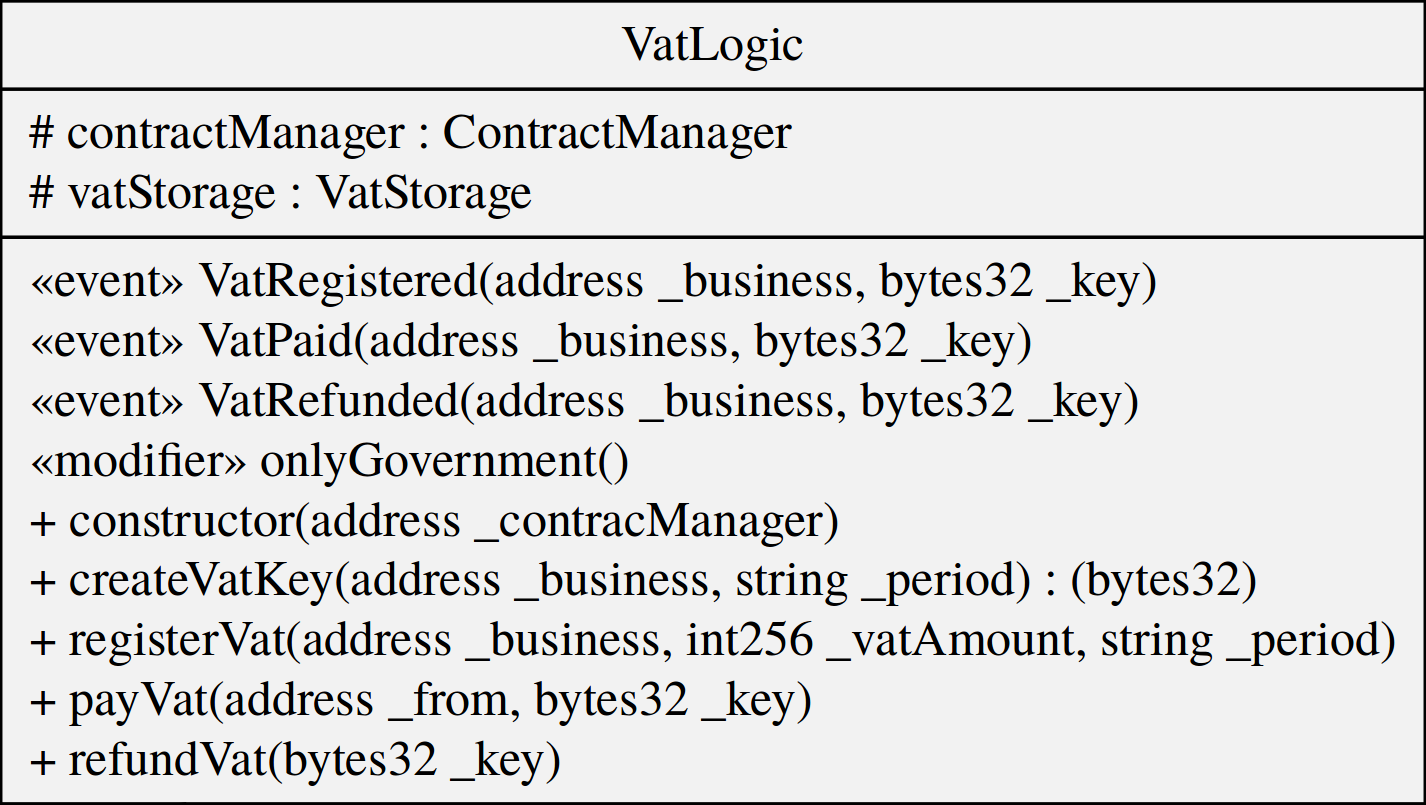
\includegraphics[scale=0.20]{res/images/solidity/vatlogic.png}
	\caption{class diagram of the VatLogic contract}
\end{figure}
\pagebreak
\paragraph{OrderLogic}\mbox{}\\

\noindent This contract allows to register an order. The function \texttt{registerOrder} can be called only by the \texttt{Purchase} contract because when a purchase is made on \textit{Soldino} the latter contract is called and forwards the request to this contract. In other words, if a purchase contains products from different sellers, the \texttt{Purchase} contract calls \texttt{registerOrder} for every different seller. \\
\texttt In addition, {registerOrder}  registers the VAT movements related to the businesses involved in the purchase.
\begin{figure}[H]
	\centering
	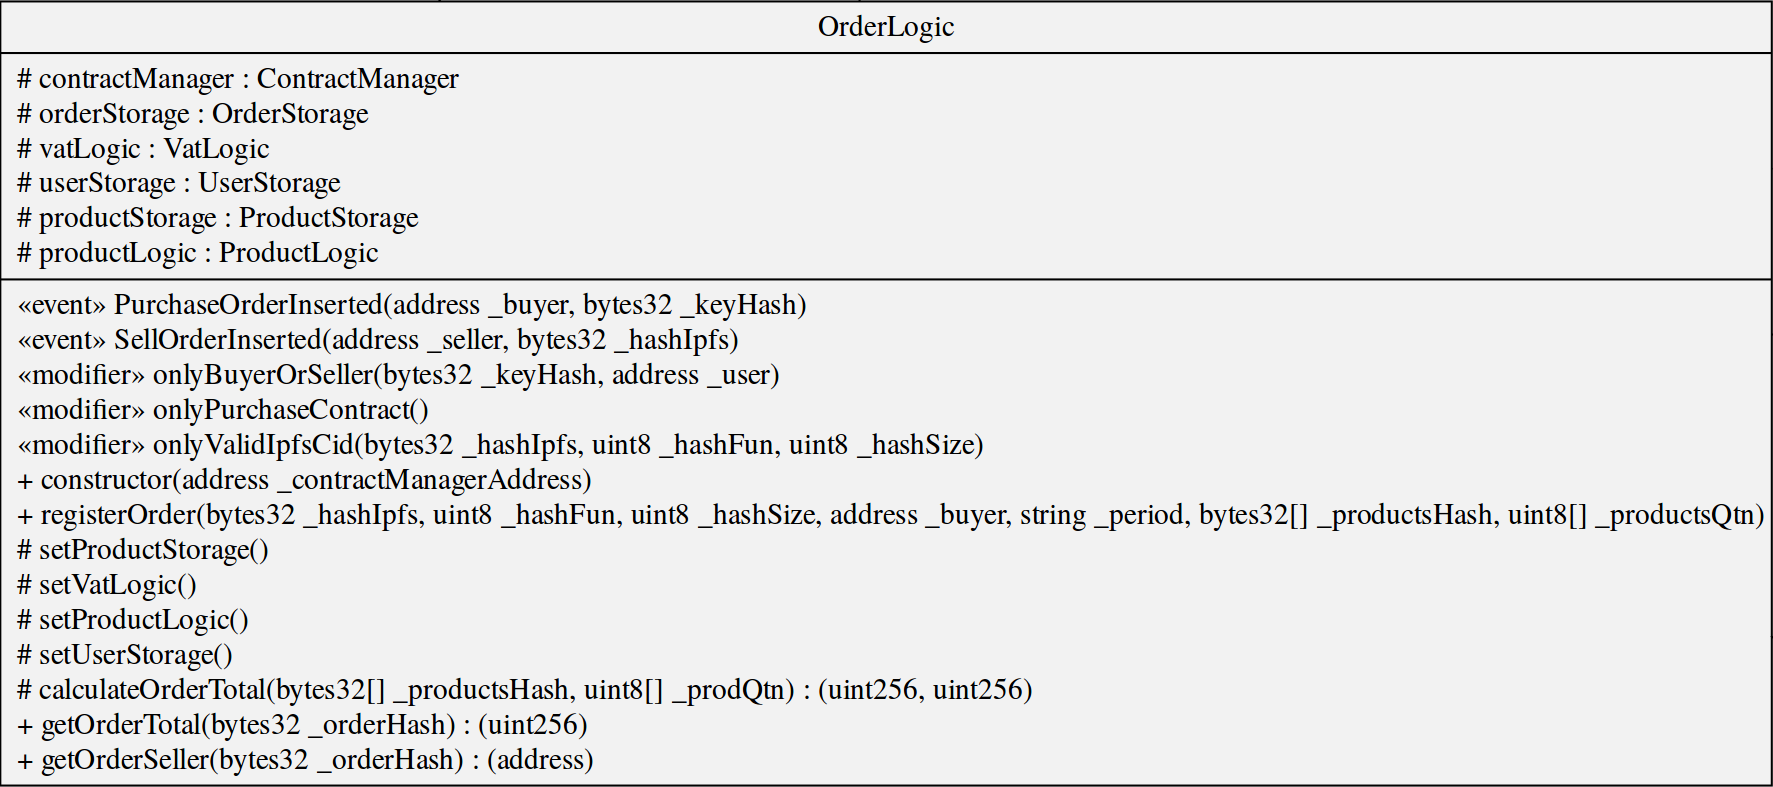
\includegraphics[scale=0.25]{res/images/solidity/orderlogic.png}
	\caption{class diagram of the OrderLogic contract}
\end{figure}